
\documentclass[crop,tikz]{standalone}
\usepackage[utf8]{inputenc}
\usepackage{tikz}
\usepackage{pgfplots}
\pgfplotsset{compat=newest}
\usepgfplotslibrary{groupplots}
\begin{document}
% This file was created by matplotlib2tikz v0.6.15.
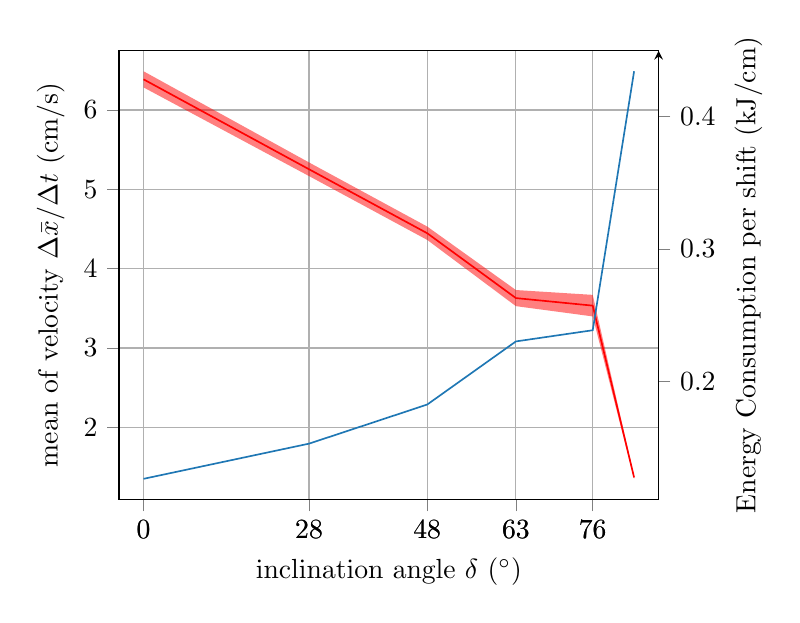
\begin{tikzpicture}

\definecolor{color0}{rgb}{0.12156862745098,0.466666666666667,0.705882352941177}

\begin{axis}[
xlabel={inclination angle $\delta$ ($^\circ$)},
ylabel={mean of velocity $\Delta \bar{x} / \Delta t$ (cm/s)},
xmin=-4.15, xmax=87.15,
ymin=1.09414576089746, ymax=6.74564551738317,
tick align=outside,
tick pos=left,
xmajorgrids,
x grid style={lightgray!92.026143790849673!black},
ymajorgrids,
y grid style={lightgray!92.026143790849673!black},
xtick={0, 28, 48, 63, 76}
]
\path [fill=red, fill opacity=0.5] (axis cs:0,6.28528123071327)
--(axis cs:0,6.48875916481564)
--(axis cs:28,5.33934266652788)
--(axis cs:48,4.53114336159411)
--(axis cs:63,3.7309637886084)
--(axis cs:76,3.66994129660673)
--(axis cs:83,1.3851046509481)
--(axis cs:83,1.35103211346499)
--(axis cs:83,1.35103211346499)
--(axis cs:76,3.39833929573204)
--(axis cs:63,3.52776760577565)
--(axis cs:48,4.36257320552257)
--(axis cs:28,5.16755408859268)
--(axis cs:0,6.28528123071327)
--cycle;

\addplot [semithick, red, forget plot]
table {%
0 6.38702019776445
28 5.25344837756028
48 4.44685828355834
63 3.62936569719202
76 3.53414029616939
83 1.36806838220655
};
\end{axis}

\begin{axis}[
ylabel={Energy Consumption per shift (kJ/cm)},
xmin=-4.15, xmax=87.15,
ymin=0.111533097040484, ymax=0.449231403084515,
axis y line=right,
tick align=outside,
xtick pos=left,
ytick pos=right,
x grid style={lightgray!92.026143790849673!black},
y grid style={lightgray!92.026143790849673!black},
xtick={0, 28, 48, 63, 76}
]
\addplot [semithick, color0, forget plot]
table {%
0 0.126883020042485
28 0.153380329929775
48 0.182836377984336
63 0.230379485946148
76 0.238816506654597
83 0.433881480082513
};
\end{axis}

\end{tikzpicture}
%% End matplotlib2tikz content %% 
\end{document}